\chapter{Dataset}

\section{Generator input parameters}

We were able to create a large dataset using the generator. More specifically, we set the input parameters of the generator to the following values:

\begin{center}
 chkNumMean = 5 chkNumStDev = 2
\end{center}

The number of daily check-ins will be random and 95\% of these random values will be between 1 and 9, according to the 3-sigma empirical rule for the normal 
distribution. 

\begin{center}
 chkDurMean = 2 chkDurStDev = 0.1
\end{center}

The duration of each visit will be random and 95\% of these random values will be between 1.8 and 2.2 hours.

\begin{center}
 maxDist = 50000.0 dist = 500.0
\end{center}

Each user will be able to visit places that are in 50000 meters radius from his home or travel location. Also, he is allowed to walk in a 500 meters radius 
from the one place he visits to the next one.

\begin{center}
 startTime = 9 endTime = 23
\end{center}

Each user will visit the first place of the day at 9 am. Moreover, the last daily check-in should take place no later than 11 pm.

\begin{center}
 startDate = 01-01-2015 endDate = 03-01-2015
\end{center}

The generator will produce daily routes for the time period between the 1st of January 2015 and the 1st of March 2015. \\

Therefore, the generator run with the specific input parameters in order to create a large dataset of users and their respective daily routes. 

\section{Generator execution architecture}

Respecting the request restrictions for the users of the free Google Directions API to 2500 requests per day to the API, the generator could run 
once a day creating 14 users at a time for the specific input parameters. Therefore, we set up a cluster of 31 Virtual Machines (VMs) in order to be able to create a much 
bigger number of users per day. Each VM of the cluster had 1 CPU, 1 GB RAM and 10 GB disk. The cluster used recourses located at the Computing 
Systems Laboratory at NTUA. The PostgreSQL database, where the source data were stored, was set up in a different VM where the 
generator run as well. This specific VM had 2 CPU, 4 GB RAM and 40 GB disk in order to be able to store the source data. When the generator was running 
on the cluster VMs, a remote connection to the PostgreSQL database was established in order to gain access to the source data as well. 

\begin{figure}[H]
  \centering
  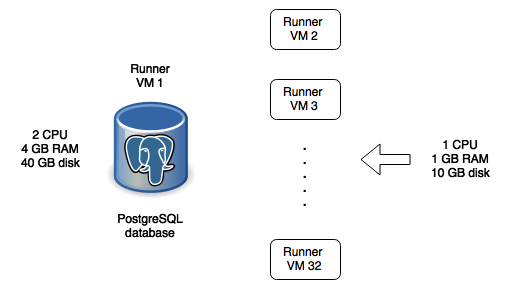
\includegraphics[width=0.8\textwidth]{figures/gen_arch.png}
  \caption{Generator execution architecture}
\end{figure}

In this way, we were able to run the generator on each VM collecting 448 users per day, creating 14 users per VM with the specified input parameters. 
At the end of the generator's run period, we were able to have 9464 users and their 2 months daily routes. 
The created dataset was available in the generator's two output files, one that stored the user's daily check-ins and another one having the user's total 
gps traces indicating the daily trajectories.

\section{Dataset storage model}

The dataset created by the generator consists of 641 MB data of check-ins and 2.4 GB data of GPS traces. We also had available a 14 GB friend graph which 
we adjusted in order to match the number of 9464 users created by the generator. The overall dataset of check-ins, GPS traces and friends was stored 
into an HBase distributed database using the following data model.

\subsection{Friends Table}

The data about friends consists of user ids. For example, user no.1 has friends the users no.2, no.3 etc. This information is parsed from the friend graph and 
inserted into HBase in byte form using the following schema:

\begin{itemize}
 \item Row: each row holds all the users that are friends of the user whose id is the key of the row.
 \item Column Family: there is one column family 'friends' including all the friends of one user.
 \item Column Qualifier: the qualifier that represents a single friend is the friend's user id.
\end{itemize}

\begin{table}[H]
\begin{center}
\begin{tabular}{|c|c|c|c|c|}
 \hline
 Row & \multicolumn{3}{|c|}{Friends} \\
 \hline
 Key & user id \#1 & user id \#2 & user id \#3 \\
 \hline
 1 & 145 & 2901 & 1204 \\ \hline 
 2 & 3423 & 1023 & 965 \\
 \hline
\end{tabular}
\end{center}
\caption{Example of HBase Table 'friends'}
\end{table}

\subsection{Check-ins Table}

The user's check-ins are parsed from the corresponding generator's output file and inserted to HBase in byte form using the following schem:

\begin{itemize}
 \item Row: each row holds all the check-ins of the user whose user id is the row key.
 \item Column Family: there is one column family 'checkIns' which holds all the check-ins of each user.
 \item Column Qualifier: the qualifier that represents a single user check-in is its timestamp.
\end{itemize}

\begin{table}[H]
\begin{center}
\begin{tabular}{|c|c|c|c|c|}
 \hline
 Row & \multicolumn{3}{|c|}{checkIns} \\
 \hline
 Key & timestamp \#1 & timestamp \#2 & timestamp \#3 \\
 \hline
 1 & 1420117200700 & 1420124471700 & 1420189200700 \\ \hline 
\end{tabular}
\end{center}
\caption{Example of HBase Table 'check-ins'}
\end{table}

\subsection{GPS traces Table}

The user's GPS traces are parsed from the corresponding generator's output file and inserted to HBase in byte form using the following schem:

\begin{itemize}
 \item Row: each row holds all the GPS traces of the user whose user id is the row key.
 \item Column Family: there is one column family 'gpsTraces' which holds all the GPS traces of each user.
 \item Column Qualifier: the qualifier that represents a single user GPS trace is the geographical coordinates and timestamp of the GPS trace.
\end{itemize}

\begin{table}[H]
\begin{center}
\begin{tabular}{|c|c|c|c|c|}
 \hline
 Row & \multicolumn{2}{|c|}{gpsTraces} \\
 \hline
 Key & qualifier \#1 & qualifier \#2\\
 \hline
 1 & (25.694, 79.836) 1420117200700 & (25.69274, 79.8394) 1420124471700 \\ \hline 
\end{tabular}
\end{center}
\caption{Example of HBase Table 'gps-traces'}
\end{table}

\section{Dataset storage architecture}

The overall dataset was stored into an HBase distributed database. The HBase was set up over HDFS on a cluster of 32 VMs, consisting of 1 master and and 32 region servers 
and 1 namenode and 32 datanodes. All different types of data were splitted into 32 parts, so that they are distributed equally into the region servers when the 
following tables were created. More specifically, when we created the table of 'friends' in HBase, we predefined the keys where the total table would be splitted 
into the region servers. Thus, the table was pre-splitted into 32 regions so that the data were equally divided into the region servers. The split into 32 parts was 
also done for the tables of 'check-ins' and 'gps-traces'. The master VM which contains the HBase master as well as the namenode has 2 CPU, 4GB RAM and 40 GB disk. 
The master is at the same time a region server and a datanode. The other 31 VMs holding the rest region servers and datanodes have 1 CPU, 2 GB RAM and 10 GB disk. 
The cluster is accomodated on a OpenStack managed cloud service located at Computing Systems Laboratory in NTUA.

\begin{figure}[H]
  \centering
  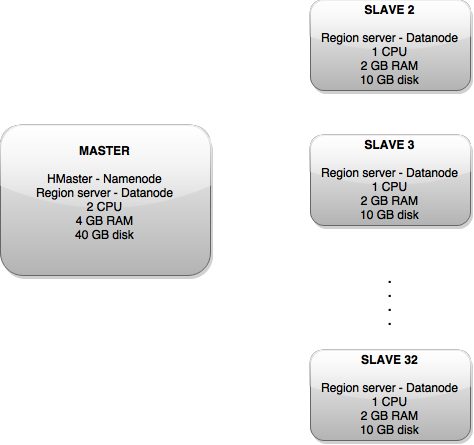
\includegraphics[width=0.6\textwidth]{figures/hbase_cluster_gray.png}
  \caption{HBase cluster architecture}
\end{figure}

